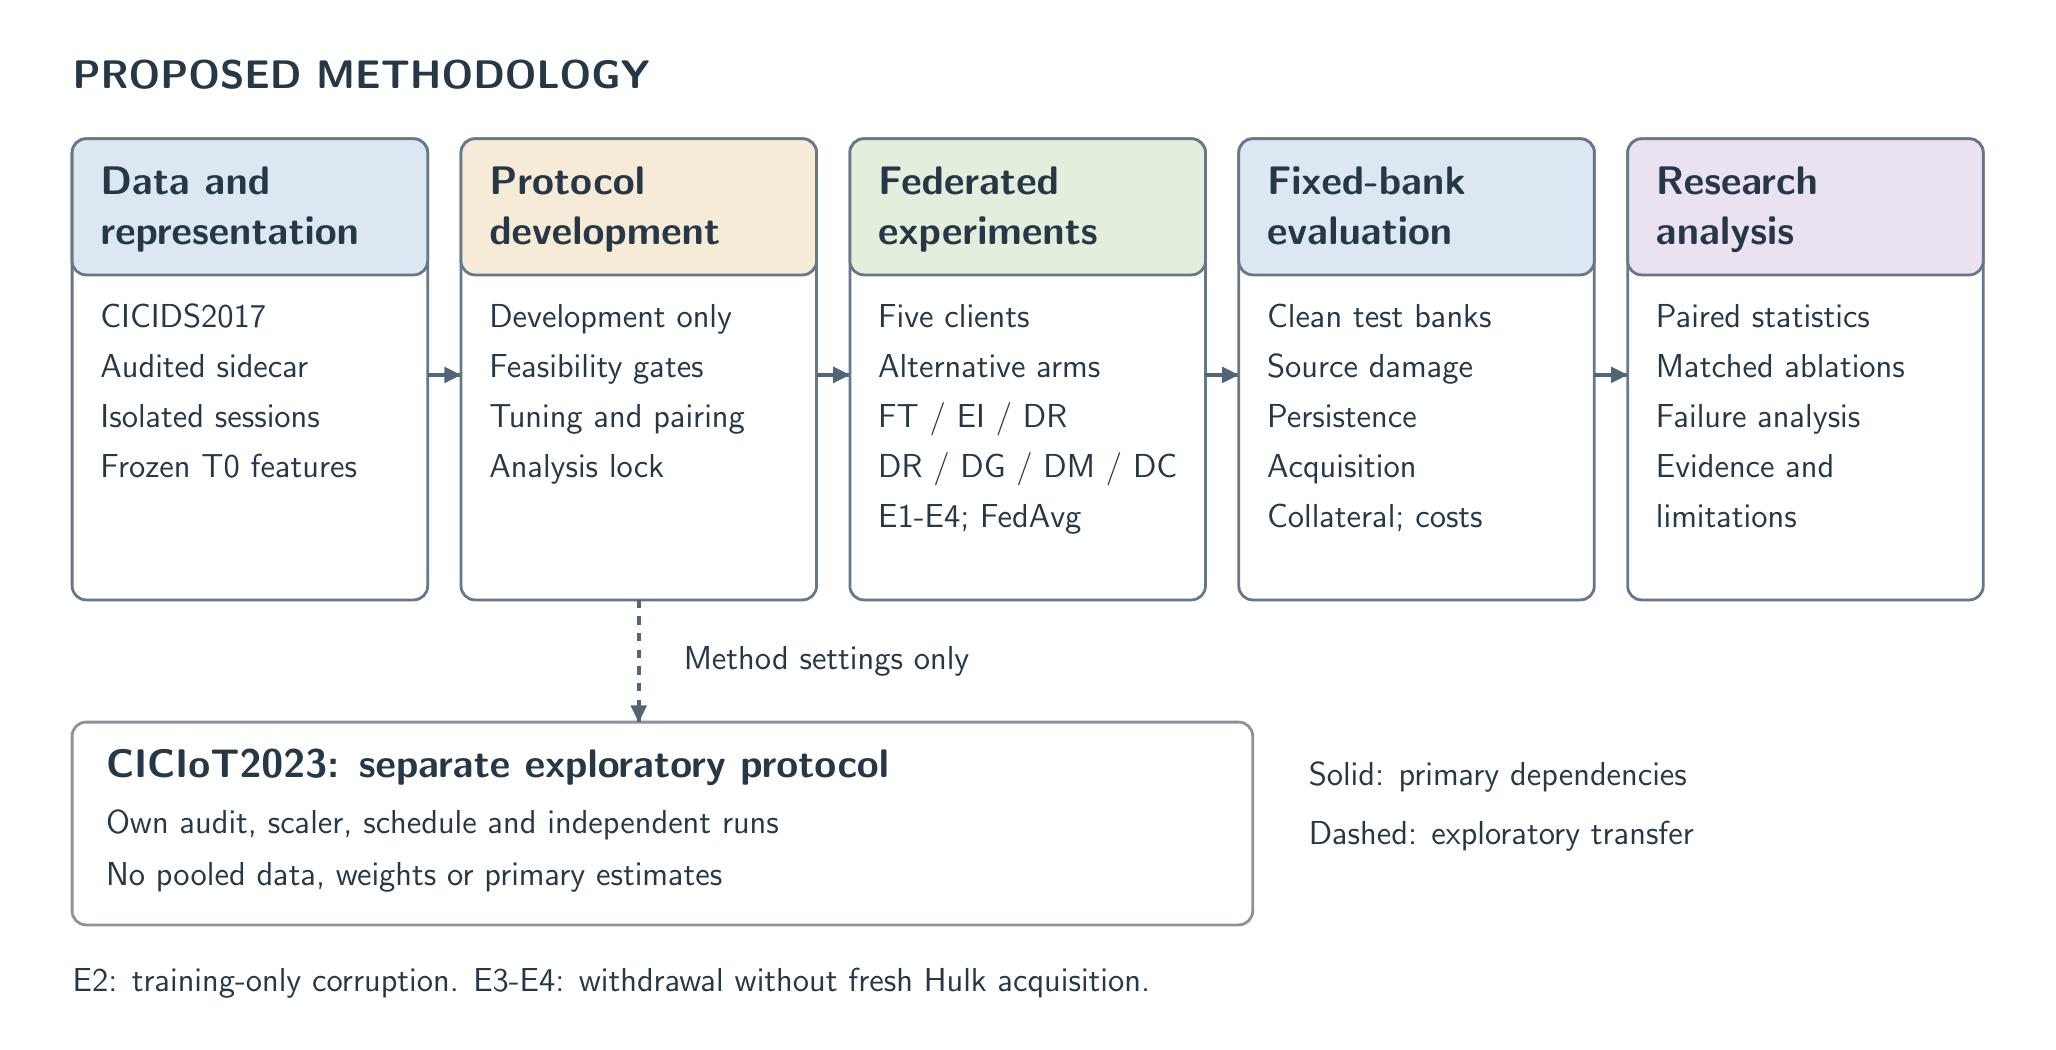
\begin{tikzpicture}[x=1bp,y=-1bp]
\path[use as bounding box] (0,0) rectangle (720,358);
\node[anchor=base west,inner sep=0,text={rgb,255:red,38;green,55;blue,70},font=\sffamily\bfseries\fontsize{15}{17.25}\selectfont] at (16,22) {PROPOSED METHODOLOGY};
\path[draw={rgb,255:red,102;green,119;blue,137},fill={rgb,255:red,255;green,255;blue,255},line width=1bp,rounded corners=5bp] (16,40) rectangle (144,206);
\path[draw={rgb,255:red,102;green,119;blue,137},fill={rgb,255:red,220;green,231;blue,242},line width=1bp,rounded corners=5bp] (16,40) rectangle (144,89);
\node[anchor=base west,inner sep=0,text={rgb,255:red,38;green,55;blue,70},font=\sffamily\bfseries\fontsize{15}{17.25}\selectfont] at (26,60) {Data and};
\node[anchor=base west,inner sep=0,text={rgb,255:red,38;green,55;blue,70},font=\sffamily\bfseries\fontsize{15}{17.25}\selectfont] at (26,78) {representation};
\node[anchor=base west,inner sep=0,text={rgb,255:red,38;green,55;blue,70},font=\sffamily\fontsize{12}{13.799999999999999}\selectfont] at (26,108) {CICIDS2017};
\node[anchor=base west,inner sep=0,text={rgb,255:red,38;green,55;blue,70},font=\sffamily\fontsize{12}{13.799999999999999}\selectfont] at (26,126) {Audited sidecar};
\node[anchor=base west,inner sep=0,text={rgb,255:red,38;green,55;blue,70},font=\sffamily\fontsize{12}{13.799999999999999}\selectfont] at (26,144) {Isolated sessions};
\node[anchor=base west,inner sep=0,text={rgb,255:red,38;green,55;blue,70},font=\sffamily\fontsize{12}{13.799999999999999}\selectfont] at (26,162) {Frozen T0 features};
\path[draw={rgb,255:red,80;green,101;blue,118},line width=1.4bp] (144,125) -- (156,125);
\path[fill={rgb,255:red,80;green,101;blue,118}] (156.000,125.000) -- (150.000,122.000) -- (150.000,128.000) -- cycle;
\path[draw={rgb,255:red,102;green,119;blue,137},fill={rgb,255:red,255;green,255;blue,255},line width=1bp,rounded corners=5bp] (156,40) rectangle (284,206);
\path[draw={rgb,255:red,102;green,119;blue,137},fill={rgb,255:red,245;green,235;blue,215},line width=1bp,rounded corners=5bp] (156,40) rectangle (284,89);
\node[anchor=base west,inner sep=0,text={rgb,255:red,38;green,55;blue,70},font=\sffamily\bfseries\fontsize{15}{17.25}\selectfont] at (166,60) {Protocol};
\node[anchor=base west,inner sep=0,text={rgb,255:red,38;green,55;blue,70},font=\sffamily\bfseries\fontsize{15}{17.25}\selectfont] at (166,78) {development};
\node[anchor=base west,inner sep=0,text={rgb,255:red,38;green,55;blue,70},font=\sffamily\fontsize{12}{13.799999999999999}\selectfont] at (166,108) {Development only};
\node[anchor=base west,inner sep=0,text={rgb,255:red,38;green,55;blue,70},font=\sffamily\fontsize{12}{13.799999999999999}\selectfont] at (166,126) {Feasibility gates};
\node[anchor=base west,inner sep=0,text={rgb,255:red,38;green,55;blue,70},font=\sffamily\fontsize{12}{13.799999999999999}\selectfont] at (166,144) {Tuning and pairing};
\node[anchor=base west,inner sep=0,text={rgb,255:red,38;green,55;blue,70},font=\sffamily\fontsize{12}{13.799999999999999}\selectfont] at (166,162) {Analysis lock};
\path[draw={rgb,255:red,80;green,101;blue,118},line width=1.4bp] (284,125) -- (296,125);
\path[fill={rgb,255:red,80;green,101;blue,118}] (296.000,125.000) -- (290.000,122.000) -- (290.000,128.000) -- cycle;
\path[draw={rgb,255:red,102;green,119;blue,137},fill={rgb,255:red,255;green,255;blue,255},line width=1bp,rounded corners=5bp] (296,40) rectangle (424,206);
\path[draw={rgb,255:red,102;green,119;blue,137},fill={rgb,255:red,228;green,238;blue,221},line width=1bp,rounded corners=5bp] (296,40) rectangle (424,89);
\node[anchor=base west,inner sep=0,text={rgb,255:red,38;green,55;blue,70},font=\sffamily\bfseries\fontsize{15}{17.25}\selectfont] at (306,60) {Federated};
\node[anchor=base west,inner sep=0,text={rgb,255:red,38;green,55;blue,70},font=\sffamily\bfseries\fontsize{15}{17.25}\selectfont] at (306,78) {experiments};
\node[anchor=base west,inner sep=0,text={rgb,255:red,38;green,55;blue,70},font=\sffamily\fontsize{12}{13.799999999999999}\selectfont] at (306,108) {Five clients};
\node[anchor=base west,inner sep=0,text={rgb,255:red,38;green,55;blue,70},font=\sffamily\fontsize{12}{13.799999999999999}\selectfont] at (306,126) {Alternative arms};
\node[anchor=base west,inner sep=0,text={rgb,255:red,38;green,55;blue,70},font=\sffamily\fontsize{12}{13.799999999999999}\selectfont] at (306,144) {FT / EI / DR};
\node[anchor=base west,inner sep=0,text={rgb,255:red,38;green,55;blue,70},font=\sffamily\fontsize{12}{13.799999999999999}\selectfont] at (306,162) {DR / DG / DM / DC};
\node[anchor=base west,inner sep=0,text={rgb,255:red,38;green,55;blue,70},font=\sffamily\fontsize{12}{13.799999999999999}\selectfont] at (306,180) {E1-E4; FedAvg};
\path[draw={rgb,255:red,80;green,101;blue,118},line width=1.4bp] (424,125) -- (436,125);
\path[fill={rgb,255:red,80;green,101;blue,118}] (436.000,125.000) -- (430.000,122.000) -- (430.000,128.000) -- cycle;
\path[draw={rgb,255:red,102;green,119;blue,137},fill={rgb,255:red,255;green,255;blue,255},line width=1bp,rounded corners=5bp] (436,40) rectangle (564,206);
\path[draw={rgb,255:red,102;green,119;blue,137},fill={rgb,255:red,220;green,231;blue,242},line width=1bp,rounded corners=5bp] (436,40) rectangle (564,89);
\node[anchor=base west,inner sep=0,text={rgb,255:red,38;green,55;blue,70},font=\sffamily\bfseries\fontsize{15}{17.25}\selectfont] at (446,60) {Fixed-bank};
\node[anchor=base west,inner sep=0,text={rgb,255:red,38;green,55;blue,70},font=\sffamily\bfseries\fontsize{15}{17.25}\selectfont] at (446,78) {evaluation};
\node[anchor=base west,inner sep=0,text={rgb,255:red,38;green,55;blue,70},font=\sffamily\fontsize{12}{13.799999999999999}\selectfont] at (446,108) {Clean test banks};
\node[anchor=base west,inner sep=0,text={rgb,255:red,38;green,55;blue,70},font=\sffamily\fontsize{12}{13.799999999999999}\selectfont] at (446,126) {Source damage};
\node[anchor=base west,inner sep=0,text={rgb,255:red,38;green,55;blue,70},font=\sffamily\fontsize{12}{13.799999999999999}\selectfont] at (446,144) {Persistence};
\node[anchor=base west,inner sep=0,text={rgb,255:red,38;green,55;blue,70},font=\sffamily\fontsize{12}{13.799999999999999}\selectfont] at (446,162) {Acquisition};
\node[anchor=base west,inner sep=0,text={rgb,255:red,38;green,55;blue,70},font=\sffamily\fontsize{12}{13.799999999999999}\selectfont] at (446,180) {Collateral; costs};
\path[draw={rgb,255:red,80;green,101;blue,118},line width=1.4bp] (564,125) -- (576,125);
\path[fill={rgb,255:red,80;green,101;blue,118}] (576.000,125.000) -- (570.000,122.000) -- (570.000,128.000) -- cycle;
\path[draw={rgb,255:red,102;green,119;blue,137},fill={rgb,255:red,255;green,255;blue,255},line width=1bp,rounded corners=5bp] (576,40) rectangle (704,206);
\path[draw={rgb,255:red,102;green,119;blue,137},fill={rgb,255:red,234;green,226;blue,241},line width=1bp,rounded corners=5bp] (576,40) rectangle (704,89);
\node[anchor=base west,inner sep=0,text={rgb,255:red,38;green,55;blue,70},font=\sffamily\bfseries\fontsize{15}{17.25}\selectfont] at (586,60) {Research};
\node[anchor=base west,inner sep=0,text={rgb,255:red,38;green,55;blue,70},font=\sffamily\bfseries\fontsize{15}{17.25}\selectfont] at (586,78) {analysis};
\node[anchor=base west,inner sep=0,text={rgb,255:red,38;green,55;blue,70},font=\sffamily\fontsize{12}{13.799999999999999}\selectfont] at (586,108) {Paired statistics};
\node[anchor=base west,inner sep=0,text={rgb,255:red,38;green,55;blue,70},font=\sffamily\fontsize{12}{13.799999999999999}\selectfont] at (586,126) {Matched ablations};
\node[anchor=base west,inner sep=0,text={rgb,255:red,38;green,55;blue,70},font=\sffamily\fontsize{12}{13.799999999999999}\selectfont] at (586,144) {Failure analysis};
\node[anchor=base west,inner sep=0,text={rgb,255:red,38;green,55;blue,70},font=\sffamily\fontsize{12}{13.799999999999999}\selectfont] at (586,162) {Evidence and};
\node[anchor=base west,inner sep=0,text={rgb,255:red,38;green,55;blue,70},font=\sffamily\fontsize{12}{13.799999999999999}\selectfont] at (586,180) {limitations};
\path[draw={rgb,255:red,137;green,147;blue,157},fill={rgb,255:red,255;green,255;blue,255},line width=1bp,rounded corners=5bp] (16,250) rectangle (441,323);
\node[anchor=base west,inner sep=0,text={rgb,255:red,38;green,55;blue,70},font=\sffamily\bfseries\fontsize{15}{17.25}\selectfont] at (28,270) {CICIoT2023: separate exploratory protocol};
\node[anchor=base west,inner sep=0,text={rgb,255:red,38;green,55;blue,70},font=\sffamily\fontsize{12}{13.799999999999999}\selectfont] at (28,290) {Own audit, scaler, schedule and independent runs};
\node[anchor=base west,inner sep=0,text={rgb,255:red,38;green,55;blue,70},font=\sffamily\fontsize{12}{13.799999999999999}\selectfont] at (28,309) {No pooled data, weights or primary estimates};
\path[draw={rgb,255:red,80;green,101;blue,118},line width=1.4bp,dashed] (220,206) -- (220,250);
\path[fill={rgb,255:red,80;green,101;blue,118}] (220.000,250.000) -- (223.000,244.000) -- (217.000,244.000) -- cycle;
\node[anchor=base west,inner sep=0,text={rgb,255:red,38;green,55;blue,70},font=\sffamily\fontsize{12}{13.799999999999999}\selectfont] at (236,231) {Method settings only};
\node[anchor=base west,inner sep=0,text={rgb,255:red,38;green,55;blue,70},font=\sffamily\fontsize{12}{13.799999999999999}\selectfont] at (461,273) {Solid: primary dependencies};
\node[anchor=base west,inner sep=0,text={rgb,255:red,38;green,55;blue,70},font=\sffamily\fontsize{12}{13.799999999999999}\selectfont] at (461,294) {Dashed: exploratory transfer};
\node[anchor=base west,inner sep=0,text={rgb,255:red,38;green,55;blue,70},font=\sffamily\fontsize{12}{13.799999999999999}\selectfont] at (16,347) {E2: training-only corruption. E3-E4: withdrawal without fresh Hulk acquisition.};
\end{tikzpicture}